% ASSIGNMENT 4 FIXED AND ADAPTIVE OPTIMAL FILTERING

\section{Fixed and Adaptive Optimal Filtering}

\lhead{Advanced Signal Processing}
\rhead{Fixed and Adaptive Optimal Filtering}

% 4.1 Wiener filter
\subsection{Wiener filter}

\subsubsection{Optimal filter coefficients}

The coefficients given for the unknown system are \textbf{b} = [1 2 3 2 1] and \textbf{a} = [1]. The SNR with normalised data is given by Equation \ref{eqn:snr}.

\begin{equation}
S N R=\frac{\sigma_{y[n]}^{2}}{\sigma_{\eta[n]}^{2}}=\frac{1^{2}}{0.1^{2}}=100=20 d B
\label{eqn:snr}
\end{equation}

\noindent
The optimum Wiener filter coefficients are calculated  by Equations \ref{eqn:wiener1}-\ref{eqn:optwiener}. 

\begin{equation}
\mathbf{p}_{z x}=E\{z[n] \mathbf{x}[n]\}=\left[\begin{array}{c}
E\{z[n] x[n]\} \\
E\{z[n] x[n-1]\} \\
\vdots \\
E\left\{z[n] x\left[n-N_{w}\right]\right\}
\end{array}\right]=\left[\begin{array}{c}
r_{z x}(0) \\
r_{z x}(-1) \\
\vdots \\
r_{z x}\left(-N_{w}\right)
\end{array}\right]
\label{eqn:wiener1}
\end{equation}

\begin{equation}
\mathbf{R}_{x x}=E\left\{\mathbf{x}[n] \mathbf{x}^{T}[n]\right\}=\left[\begin{array}{cccc}
r_{x x}(0) & r_{x x}(-1) & \cdots & r_{x x}\left(-N_{w}\right) \\
r_{x x}(1) & r_{x x}(0) & \cdots & r_{x x}\left(-N_{w}+1\right) \\
\vdots & \vdots & \ddots & \vdots \\
r_{x x}\left(N_{w}\right) & r_{x x}\left(N_{w}-1\right) & \cdots & r_{x x}(0)
\end{array}\right]
\label{eqn:weiner2}
\end{equation}

\begin{equation}
    \boldsymbol{w_{opt}} = \boldsymbol{R_{xx}^{-1} \cdot p_{zx}}
    \label{eqn:optwiener}
\end{equation}

\noindent
In order to determine the optimal Wiener filter coefficients, $R_{xx}$ and $p_{zx}$ were first calculated in MATLAB and then substituted into Equation \ref{eqn:optwiener}. I determined the coefficients to be [0.2122 0.4236 0.6333 0.4237 0.2122]. These are not the same as the coefficients of the unknown system, but appear to be scaled down by a factor of $\approx$ 0.21. This is due to the normalisation of y[n]. Removing this normalisation, I obtained the coefficients [0.9989 1.9869	2.9649	1.9655	0.9944] which are very similar to the original coefficients $\boldsymbol{b}$.

\subsubsection{Effect of noise power}

The noise variance was incrementally increased from $\sigma_{n}^{2}$ = 0.1 to 10, and its effect on the SNR was investigated. The results are shown in Table \ref{Tab:noisevar}.

\begin{table}[H]
\centering
\begin{tabular}{C{3cm} C{1cm} C{1cm} C{1cm} C{1cm} C{1cm} C{1cm}}
\Xhline{2\arrayrulewidth}
\textbf{Noise variance}  & 0.1 & 1 & 2 & 4 & 8 & 10 \\ \Xhline{2\arrayrulewidth}
\textbf{SNR (dB)}  & 52.13 & 12.83 & 6.35 & 5.29 & 3.70 & 2.47\\\Xhline{2\arrayrulewidth}
\end{tabular}
\caption{SNR values for a range of noise variances.}
\label{Tab:noisevar}
\end{table}

\noindent
Subsequently, the effect of noise variance on models of filters orders was investigated. The results of this are shown in Table \ref{Tab:wienernoise}.

\begin{table}[H]
\centering
\begin{tabular}{C{4cm} C{1cm} C{1cm} C{1cm} C{1cm} C{1cm} C{1cm}}
\Xhline{2\arrayrulewidth}
\textbf{Optimum Wiener} & \multicolumn{6}{c}{\textbf{Noise variance}}\\
\textbf{Coefficient Index}  & 0.1 & 1 & 2 & 4 & 8 & 10           \\\Xhline{2\arrayrulewidth}
                \textbf{1}                                 & 1.000 & 0.984 & 1.000 & 0.935 & 0.920 & 1.046\\
                \textbf{2}                                 & 2.000 & 2.025 & 1.901 & 2.127 & 2.045 & 2.005\\
                \textbf{3}                                 & 3.000 & 3.005 & 3.041 & 3.079 & 2.786 & 3.070\\
                \textbf{4}                                 & 2.004 & 1.947 & 2.025 & 2.173 & 1.911 & 1.952\\
                \textbf{5}                                 & 1.004 & 1.011 & 0.962 & 0.889 & 1.003 & 1.014\\\Xhline{2\arrayrulewidth}
\end{tabular}
\caption{Wiener coefficient values for different noise variance.}
\label{Tab:wienernoise}
\end{table}

\noindent
It is clear from these values that increasing the noise variance increases the error of the Wiener coefficients, which is in line with what would intuitively be expected.

\subsubsection{Computational complexity}

The computational of the calculation of optimal coefficients can be analysed by evaluating Equations \ref{eqn:wiener1}-\ref{eqn:optwiener}. The matrices in Equations \ref{eqn:wiener1} and \ref{eqn:weiner2} can be calculated using symmetry properties and are therefore of complexity $\mathcal{O}(N_{w})$ (using Big-O notation). The matrix inverse in Equation \ref{eqn:optwiener} is of complexity  $\mathcal{O}(N_{w}^{3})$. Finally, the matrix in Equation W is of complexity $2\mathcal{O}(N_{w}^{2})$. Summing the complexities of these individual steps, we obtain $\mathcal{O}(N_{w}^{3})$ + $2\mathcal{O}(N_{w}^{2})$ + $\mathcal{O}(N_{w})$ + $\mathcal{O}(N_{w})$ = $\mathcal{O}(N_{w}^{3} + 2N_{w}^{2} + 2N_{w})$ $\approx$  $\mathcal{O}(N_{w}^{3})$.

% 4.2 The least mean square (LMS) algorithm
\subsection{The least mean square (LMS) algorithm}

The LMS algorithm is a simple adaptive filter which adapts the Wiener coefficients to adapt to non-stationary signals. It is defined by Equation \ref{eqn:lms}.

\begin{equation}
\boldsymbol{w}(n+1)=\boldsymbol{w}(n)+\mu e[n] x(n), \quad n=0,1, \ldots
\label{eqn:lms}
\end{equation}

\noindent
where $\mu$ is the adaptation gain which controls the stability of the algorithm, and w(0) = 0. The error e[n] is calculated as the difference between z[n] and the output of the adaptive filter $\hat{y}[n]$, given by Equations \ref{eqn:yhat} and \ref{eqn:error}.

\begin{equation}
\hat{y}[n]=\mathbf{w}^{T}(n) \mathbf{x}(n)=\sum_{m=0}^{N_{w}} w_{m}(n) x(n-m)
\label{eqn:yhat}
\end{equation}

\begin{equation}
e[n]=z[n]-\hat{y}[n]
\label{eqn:error}
\end{equation}

\subsubsection{The \code{lms()} function}

In MATLAB, I wrote a function \code{lms()} which changes Wiener filter coefficients to adapt to non-stationary signals over time by approximating the LMS estimate $\hat{y}[n]$ for the signal $z[n]$, as well as outputting the estimation error $e[n]$ and a matrix containing the evolution of the adaptive weights over time. The code for this function is shown below.

\vspace{0.2cm}

\noindent
\code{
\textcolor{blue}{function} [y\_estimate,error,coeffs] = lms(x,z,mu,order)
\\\textcolor{white}{....}N = length(x); \textcolor{green}{\% signal length}
\\\textcolor{white}{....}coeffs = zeros(order, N-1); \textcolor{green}{\% each row represents coefficient for 1 input variable}
\\\textcolor{white}{....}y\_estimate = zeros(N, 1); 
\\\textcolor{white}{....}error = zeros(N, 1); 
\\\textcolor{white}{....}\textcolor{blue}{for} i = order+1:N 
\\\textcolor{white}{........}a = coeffs(:,i-order); \textcolor{green}{\% AR coefficient}
\\\textcolor{white}{........}b = x(i:-1:i-order+1); \textcolor{green}{\% MA coefficient}
\\\textcolor{white}{........}y\_estimate(i) = a'*b;
\\\textcolor{white}{........}error(i) = z(i) - y\_estimate(i); \textcolor{green}{\% error}
\\\textcolor{white}{........}coeffs(:,i-order+1) = coeffs(:,i-order)+mu*error(i)*b; 
\\\textcolor{white}{....}\textcolor{blue}{end}
\\\textcolor{white}{.}\textcolor{blue}{ end}
}

\noindent
Applying this function to the $\boldsymbol{x}$ and $\boldsymbol{z}$ vectors in the previous section, the results shown in Figure \ref{fig:lmsdemo} are obtained.

\begin{figure}[H]
\centering
\begin{subfigure}{.4\textwidth}
  \centering
  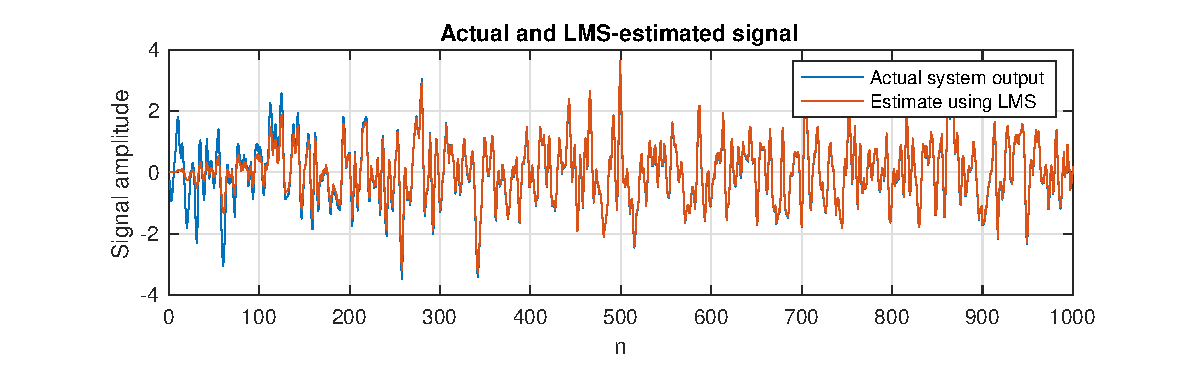
\includegraphics[width=\linewidth]{assignment4figs/actual_lms_noise01.eps}  
  \caption{Noise variance $\sigma_{n}^{2} = 0.01$.}
\end{subfigure}\\
\begin{subfigure}{.4\textwidth}
  \centering
  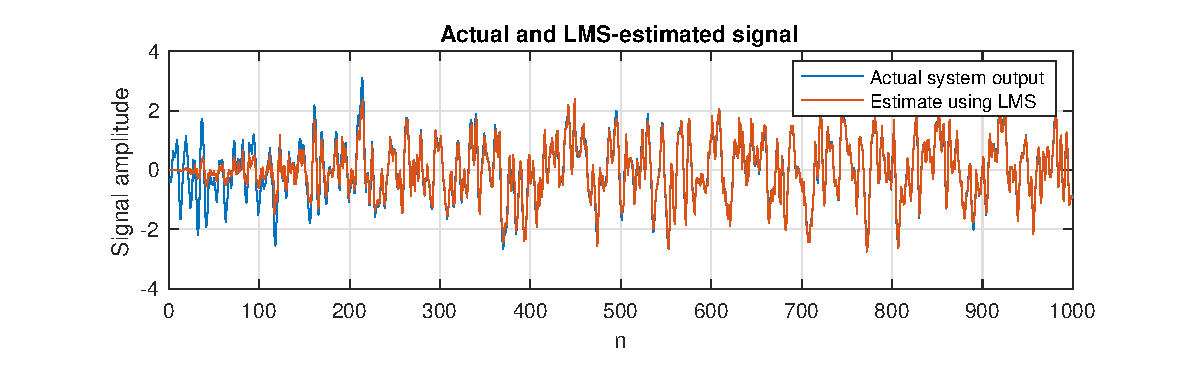
\includegraphics[width=\linewidth]{assignment4figs/actual_lms_noise1.eps}  
  \caption{Noise variance $\sigma_{n}^{2} = 1$.}
\end{subfigure}
\caption{Effect of \code{lms()} for \boldsymbol{x} and \boldsymbol{z} with variable noise variance.}
\label{fig:lmsdemo}
\end{figure}

\noindent
It is evident that the function generates coefficients which accurately estimate the system signal, but that the coefficients take longer to adapt and are less accurate for a signal with higher noise variance.

\subsubsection{Time evolution of coefficients}

Figure \ref{fig:mu} shows the evolution of the filter coefficients in time for a range of values for adaptation gain $\mu$.

\begin{figure}[H]
\centering
\begin{subfigure}{.45\textwidth}
  \centering
  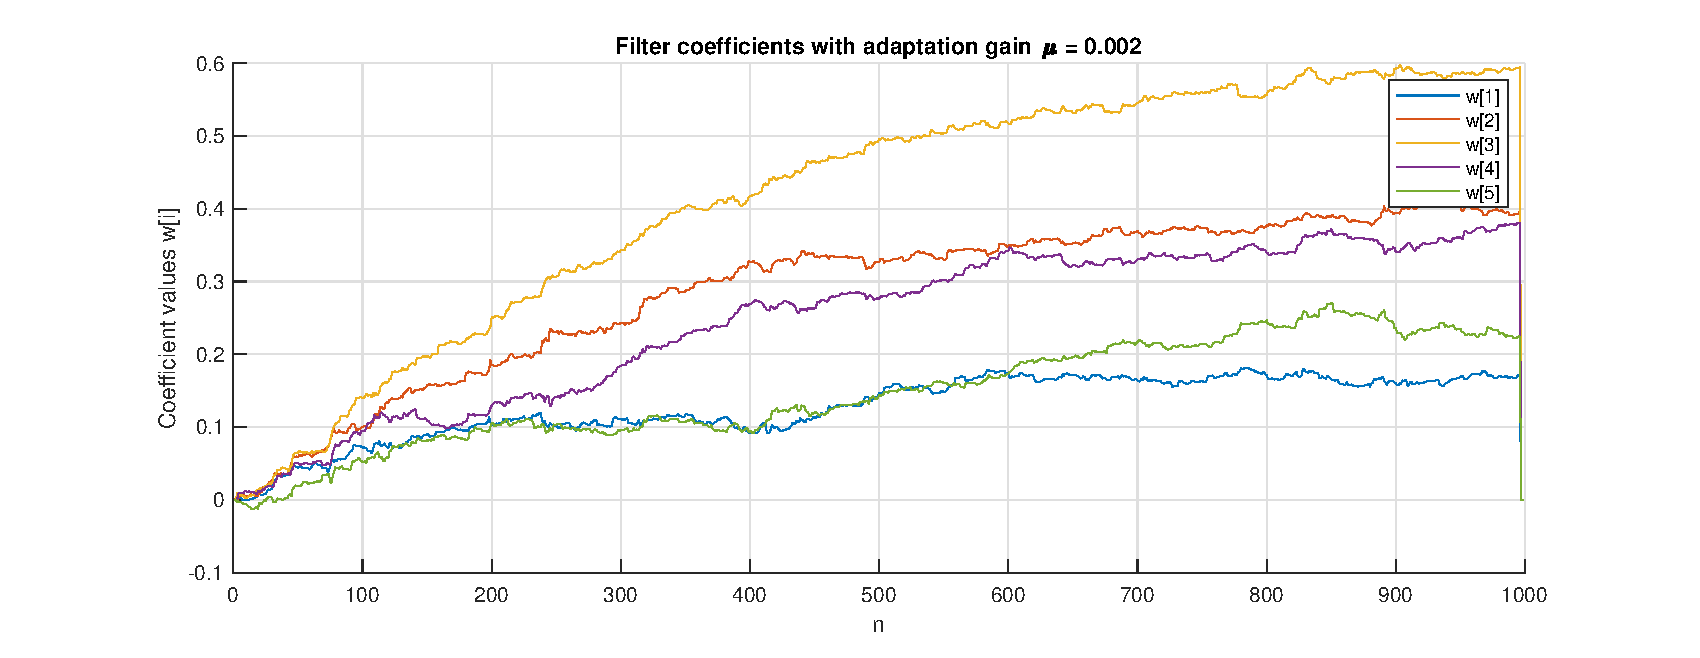
\includegraphics[width=\linewidth]{assignment4figs/mu0002.eps}
  \caption{Adaptation gain $\mu = 0.002$.}
\end{subfigure}
\begin{subfigure}{.45\textwidth}
  \centering
  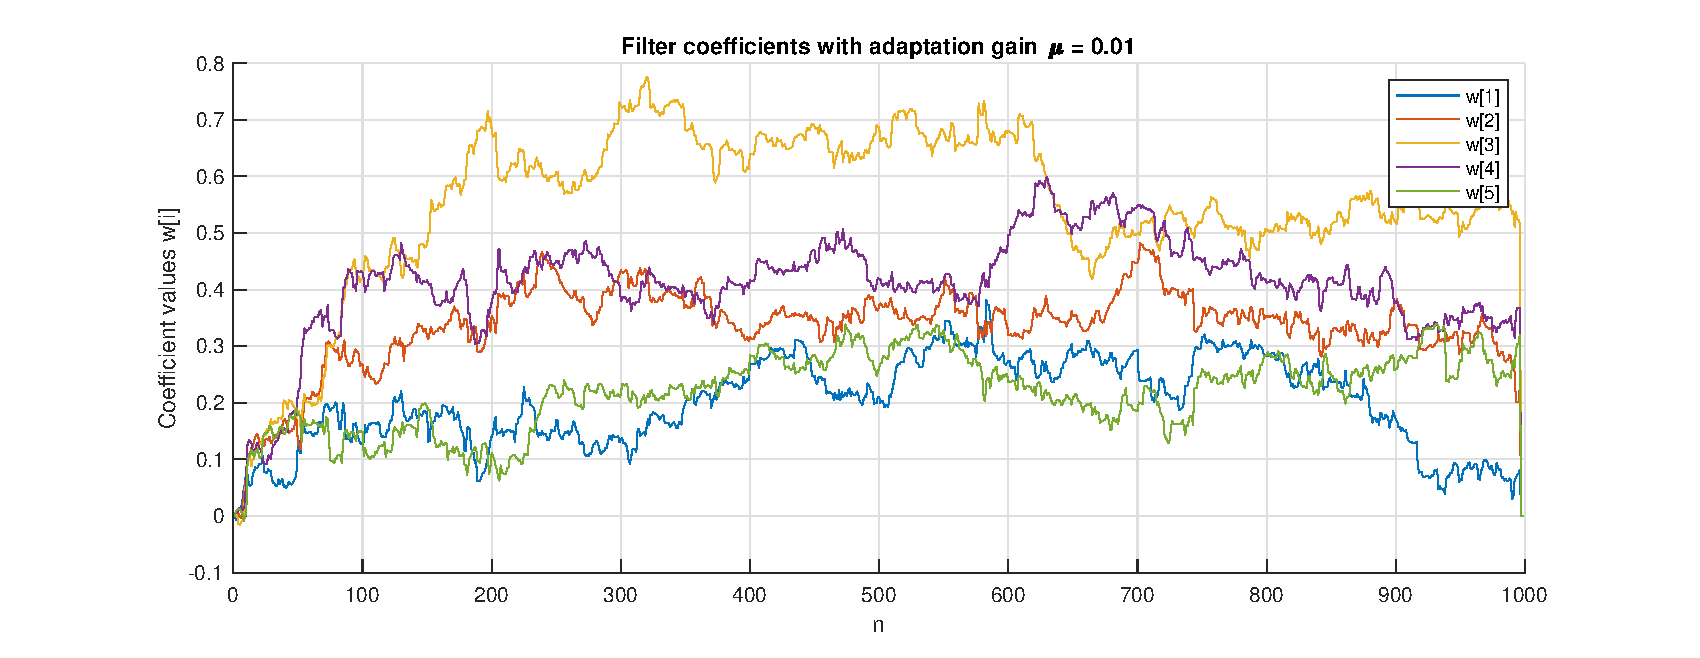
\includegraphics[width=\linewidth]{assignment4figs/mu001.eps} 
  \caption{Adaptation gain $\mu = 0.01$.}
\end{subfigure}\\
\begin{subfigure}{.45\textwidth}
  \centering
  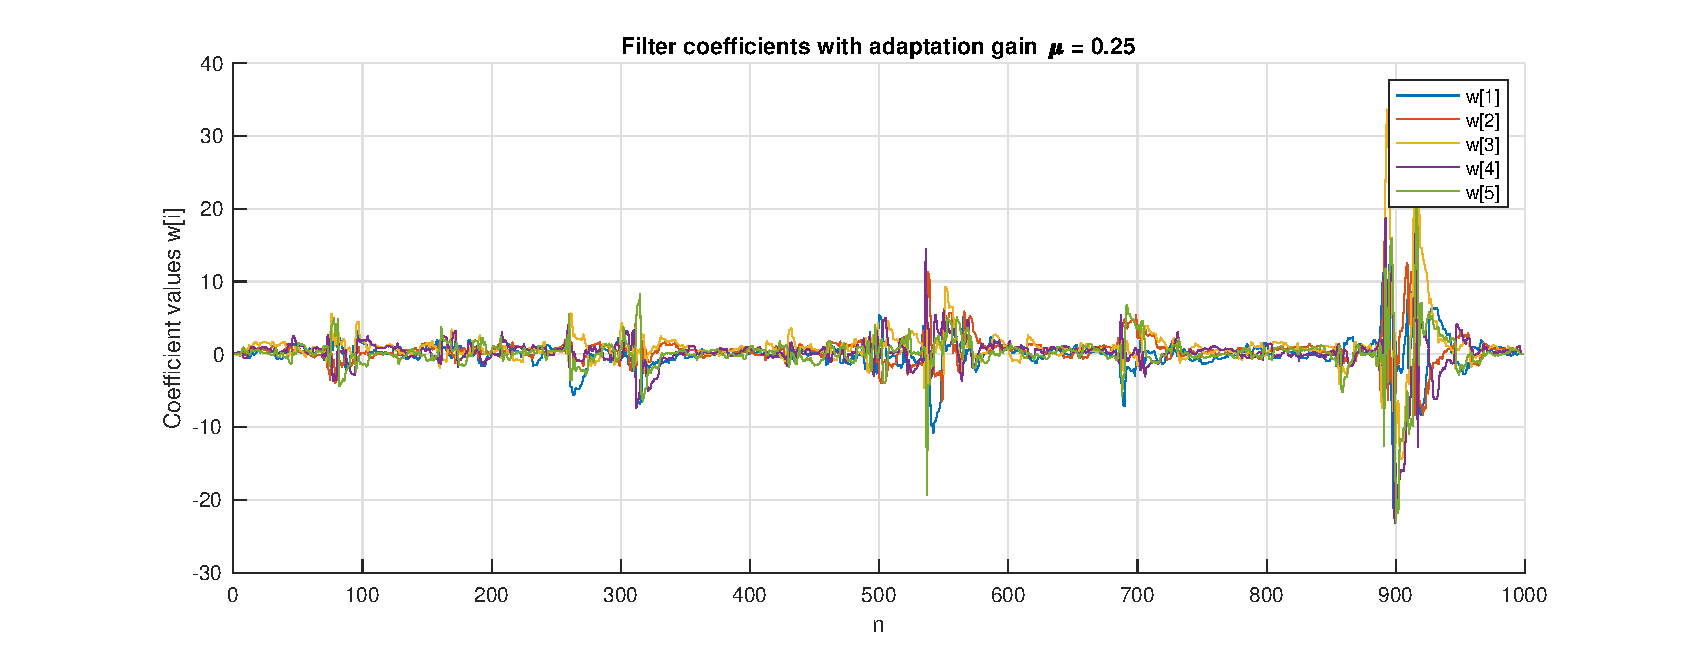
\includegraphics[width=\linewidth]{assignment4figs/mu025.eps} 
  \caption{Adaptation gain $\mu = 0.25$.}
\end{subfigure}
\begin{subfigure}{.45\textwidth}
  \centering
  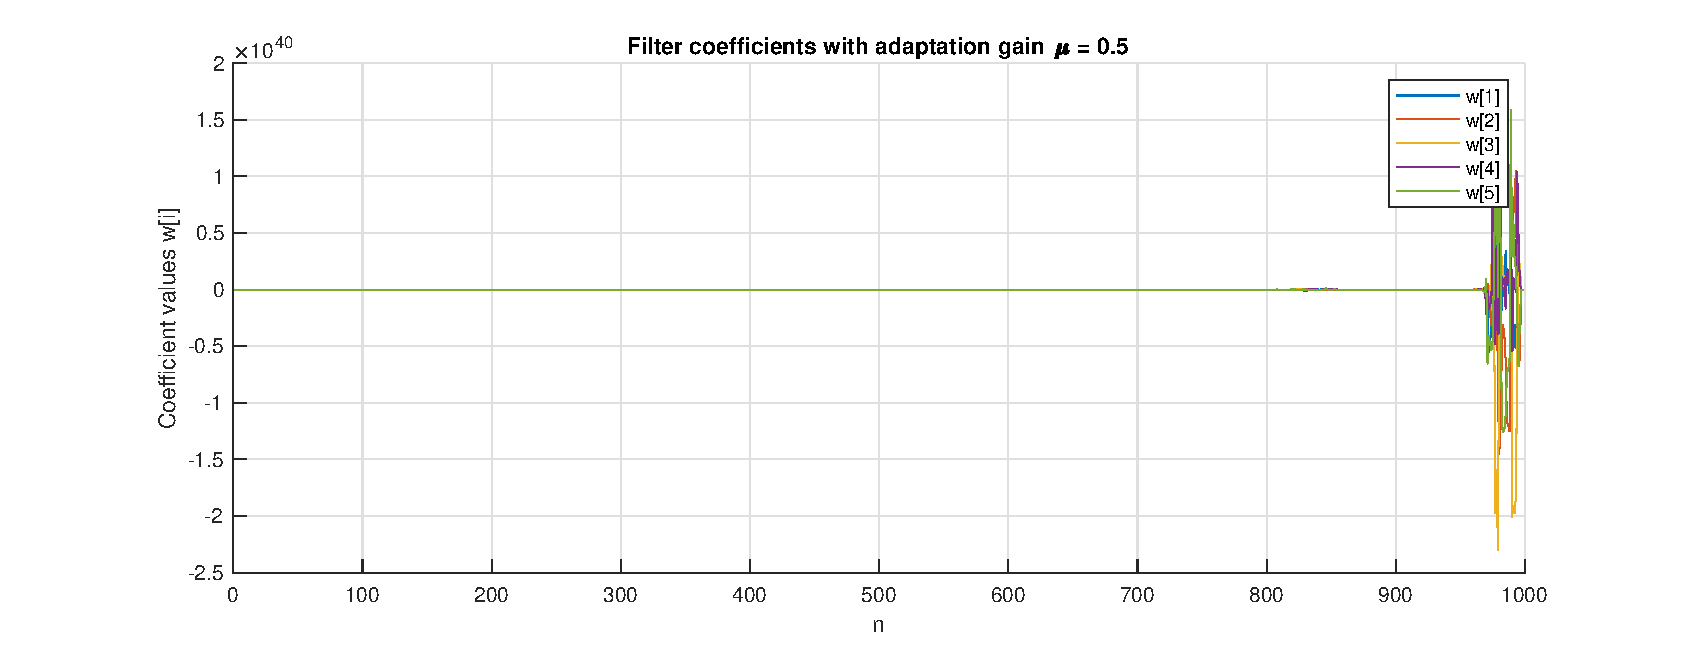
\includegraphics[width=\linewidth]{assignment4figs/mu05.eps}  
  \caption{Adaptation gain $\mu = 0.5$.}
\end{subfigure}
\caption{Coefficient evolution using \code{lms()} for variable adaptation gain $\mu$.}
\label{fig:mu}
\end{figure}

\noindent
Increasing adaptation gain $\mu$ causes the Wiener filter coefficients to converge more quickly up to a point. However, when $\mu$ is increased beyond a certain value, the coefficients actually diverge in an oscillatory and unstable manner, implying that there exists an optimum value for $\mu$ which results in fast but stable convergence.

\subsubsection{Computational complexity}

The complexity of the LMS algorithm can be analysed by evaluating Equations \ref{eqn:lms}-\ref{eqn:error}. Equation \ref{eqn:lms} has complexity $\mathcal{O}(1)$. Equation \ref{eqn:error} requires $N_{w}$ multiplications and $N_{w}+1$ additions, therefore having complexity $\mathcal{O}(2N_{w}+1)$. Finally, Equation \ref{eqn:yhat} has complexity $\mathcal{O}(2N_{w}+2)$. Therefore, the overall computational complexity is $\mathcal{O}(5N_{w}+1) \approx \mathcal{O}(N_{w})$. This algorithm has relatively low computational complexity and therefore can be utilised in adaptive filtering. 

% 4.3 Gear shifting
\subsection{Gear shifting}

Since lower adaptation gains have been found to be more effective at making coefficients converge in a stable manner, 'gear shifting' which implements time-varying adaptation gain is a sensible improvement. Gear shifting was implemented by extending the \code{lms()} function such that $\mu$ is increased by 10\% if the error signal decreases and decreased by 10\% if the error signal increases. The effect of this is shown using an initial adaptation gain $\mu$ = 0.002 in Figure \ref{fig:gearshifting}.

\begin{figure}[H]
    \centering
    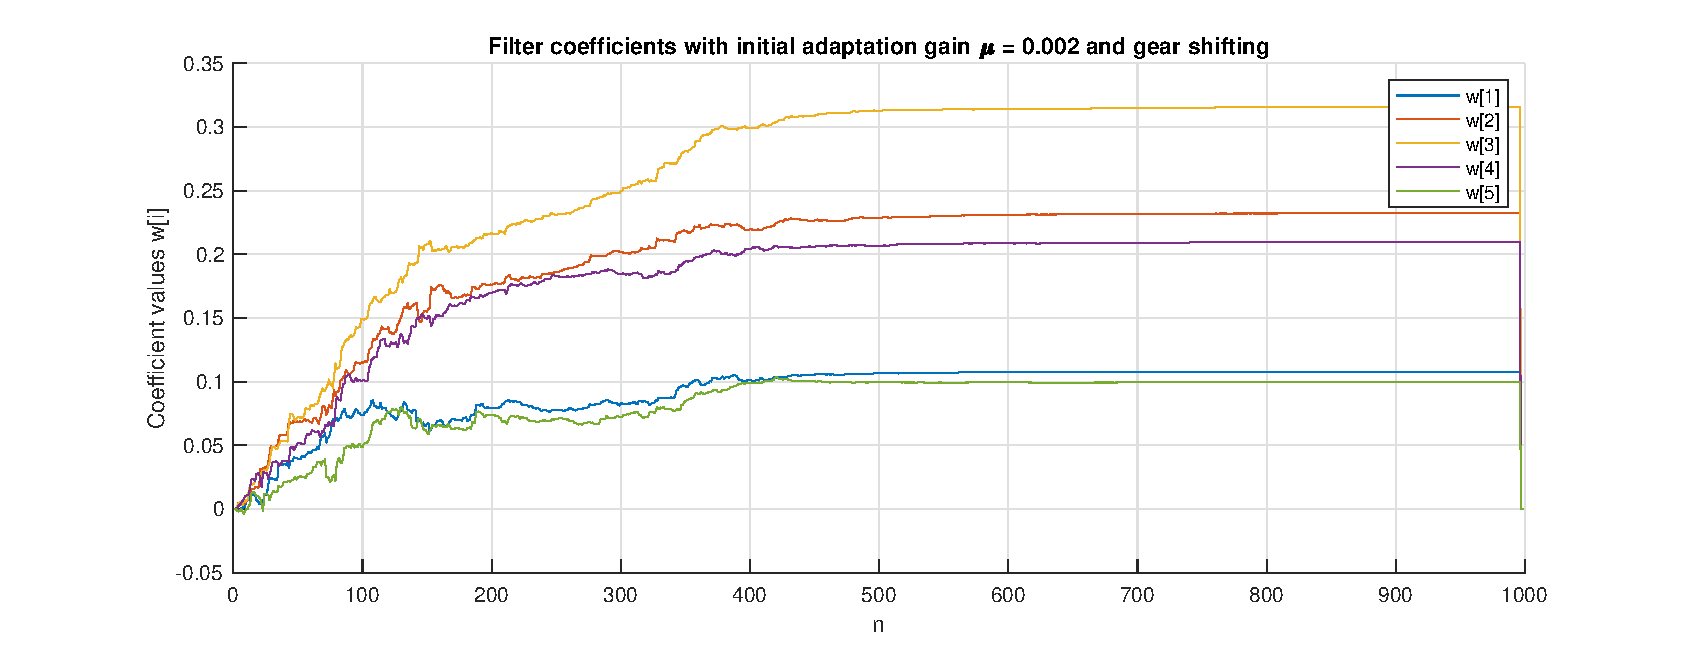
\includegraphics[width=10cm]{assignment4figs/mu002_shift.eps}
    \caption{Evolution of filter coefficients with gear shifting.}
    \label{fig:gearshifting}
\end{figure}

\noindent
This causes $\mu$ to quickly converge to an optimum value, in turn causing the filter coefficients to quickly converge to stable values as well.

% 4.4  Identification of AR processes
\subsection{Identification of AR processes}

\subsubsection{AR model implementation}

The system shown in Figure \ref{fig:sys} is an AR(2) process, therefore the LMS function needs to estimate two AR filter coefficients, $a_1$ and $a_2$. 

\begin{figure}[H]
    \centering
    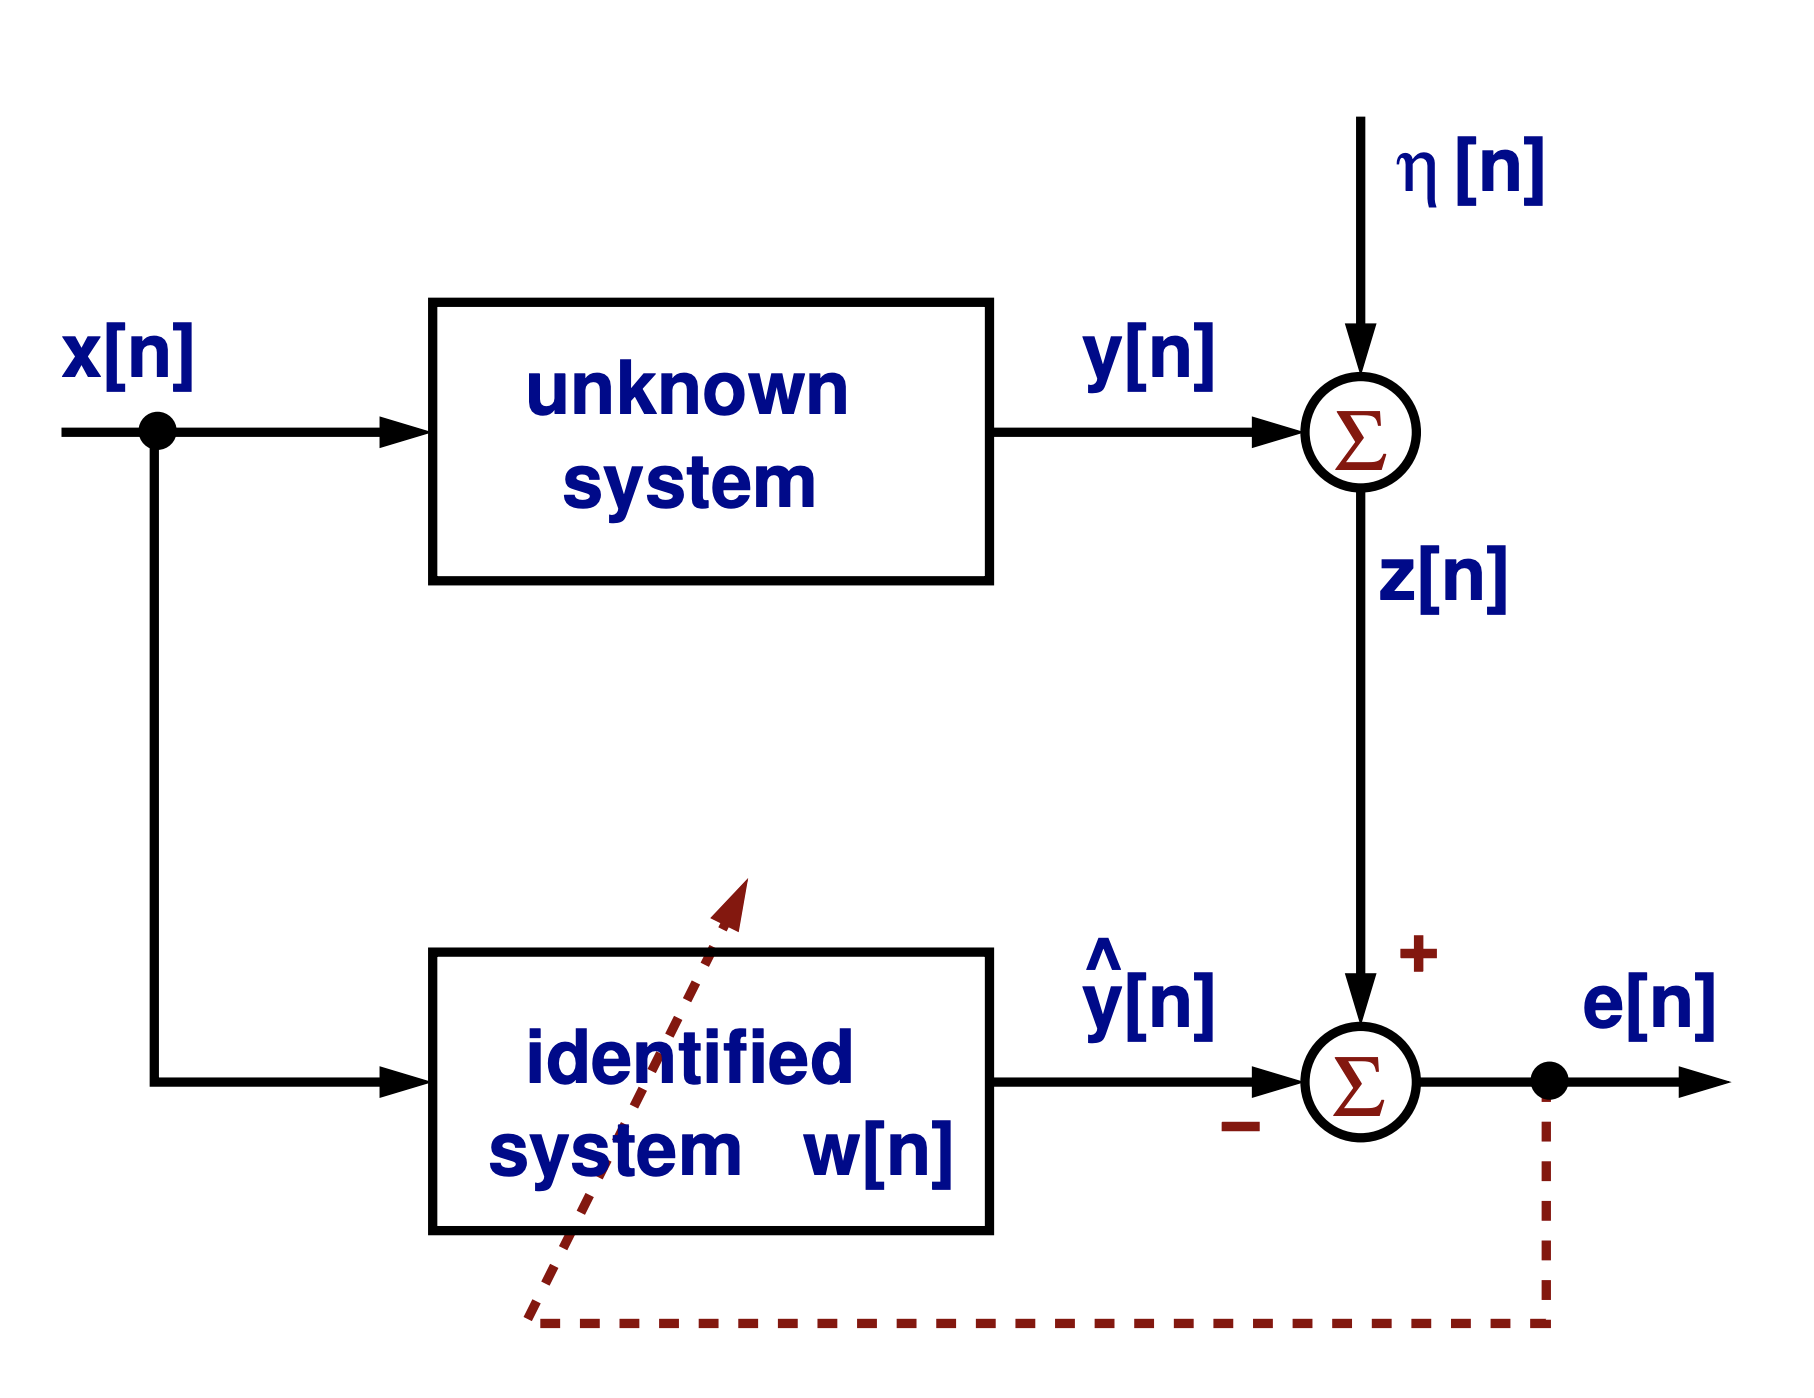
\includegraphics[width=10cm]{assignment4figs/system.png}
    \caption{System given in coursework instructions.}
    \label{fig:sys}
\end{figure}

\noindent
The given system is described by Equation \ref{eqn:ar2}.

\begin{equation}
y(n)=\sum_{i=0}^{M} b_{i} x(n-i)-\sum_{j=0}^{N} a_{j} x(n-j)=-0.9 x(n-1)-0.2 x(n-2)
\label{eqn:ar2}
\end{equation}

\noindent
Therefore, the theoretical values that we expect the coefficients to converge to are $a_1 = -0.9$ and $a_2 = -0.2$.

\subsubsection{Evolution of model coefficients}

Figure \ref{fig:mu2} shows the values of the model coefficients $a_1$ and $a_2$ using the \code{lms()} function with a range of values for adaptation gain $\mu$.

\begin{figure}[H]
\centering
\begin{subfigure}{.45\textwidth}
  \centering
  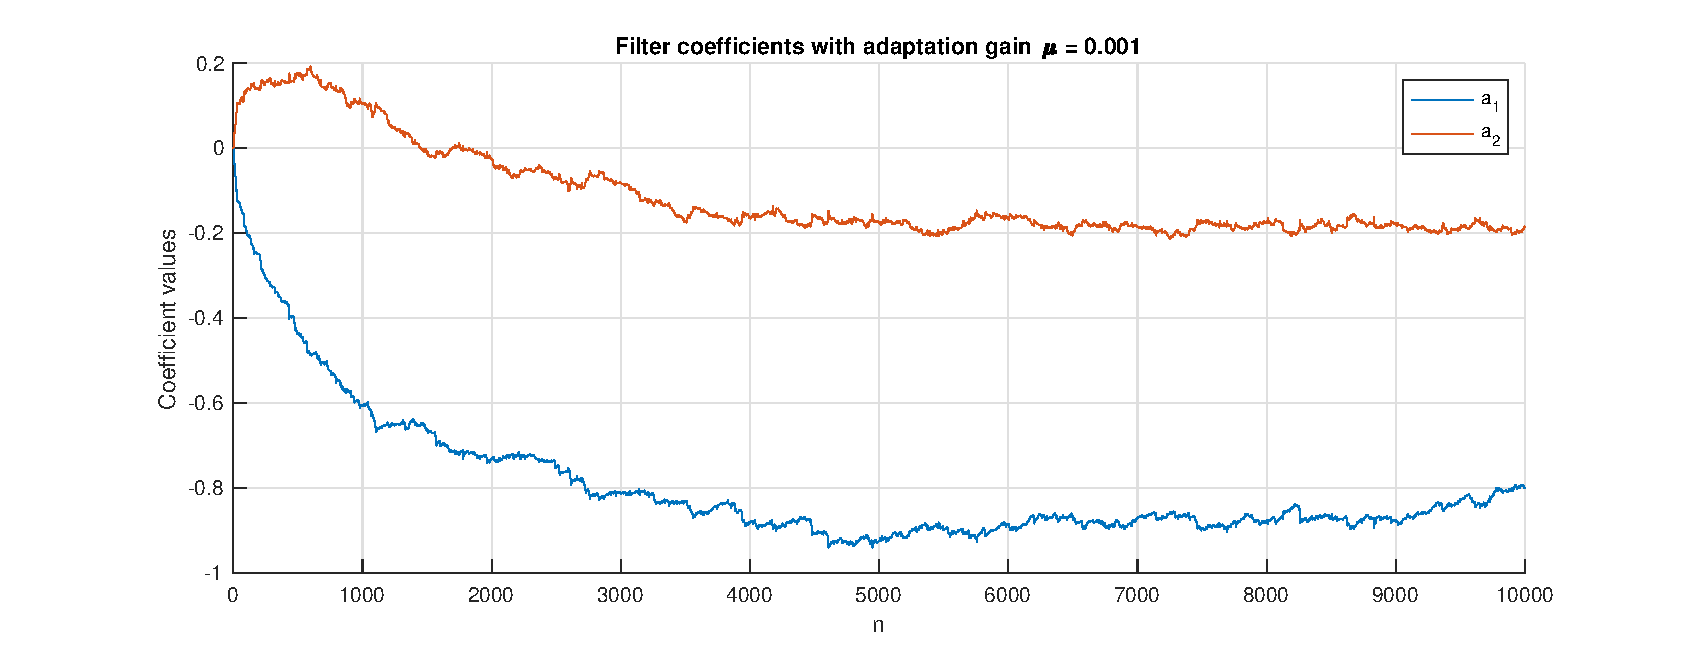
\includegraphics[width=\linewidth]{assignment4figs/armu0001.eps}
  \caption{Adaptation gain $\mu = 0.001$.}
\end{subfigure}
\begin{subfigure}{.45\textwidth}
  \centering
  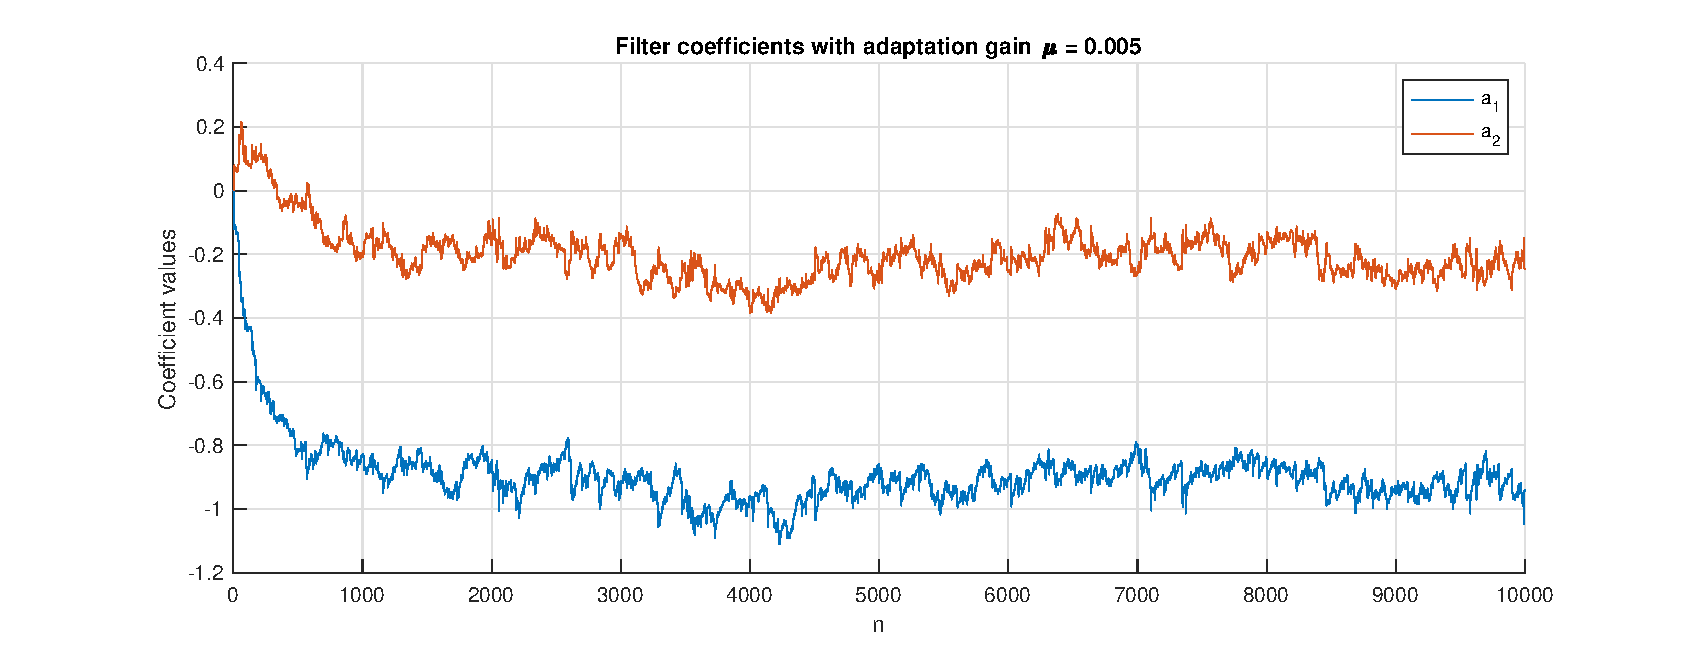
\includegraphics[width=\linewidth]{assignment4figs/armu0005.eps} 
  \caption{Adaptation gain $\mu = 0.005$.}
\end{subfigure}\\
\begin{subfigure}{.45\textwidth}
  \centering
  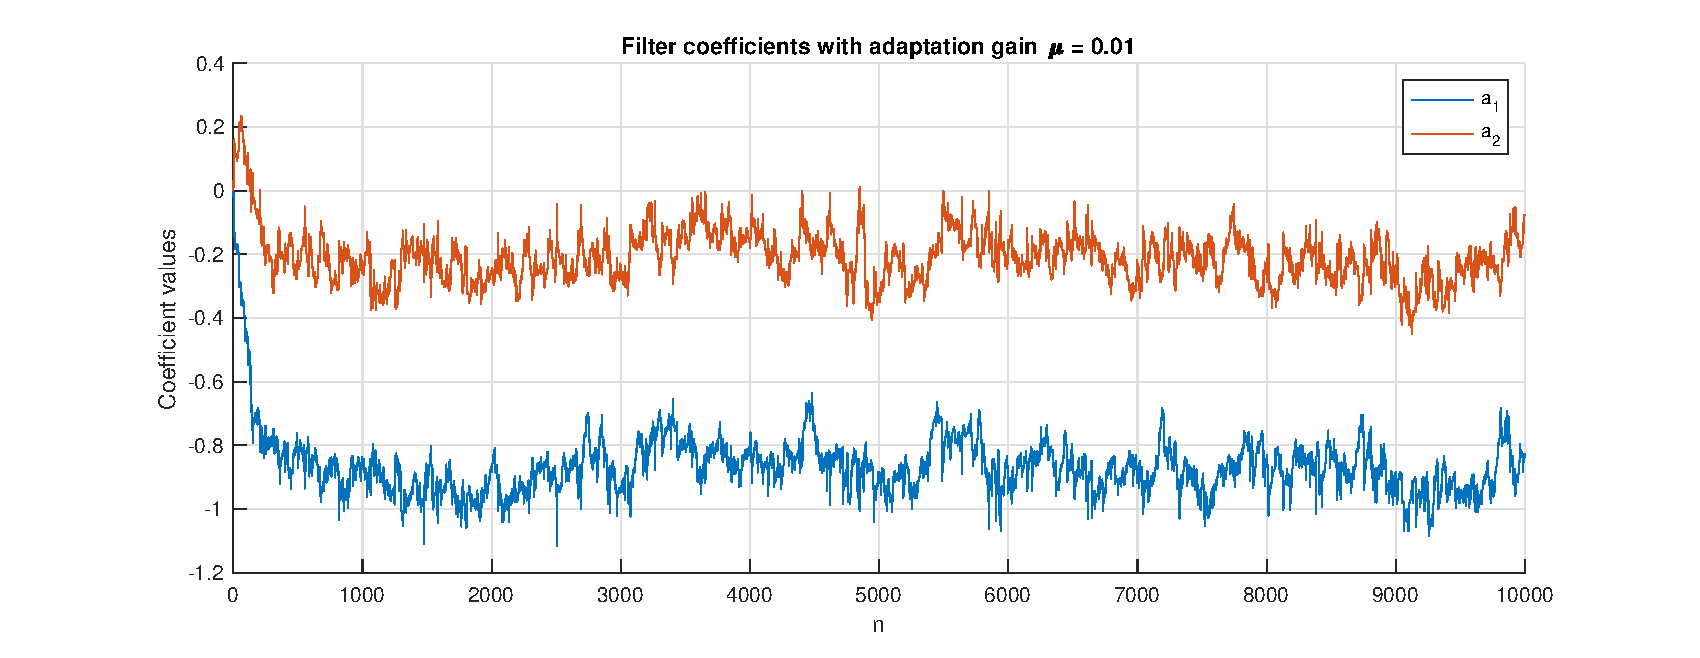
\includegraphics[width=\linewidth]{assignment4figs/armu001.eps} 
  \caption{Adaptation gain $\mu = 0.01$.}
\end{subfigure}
\begin{subfigure}{.45\textwidth}
  \centering
  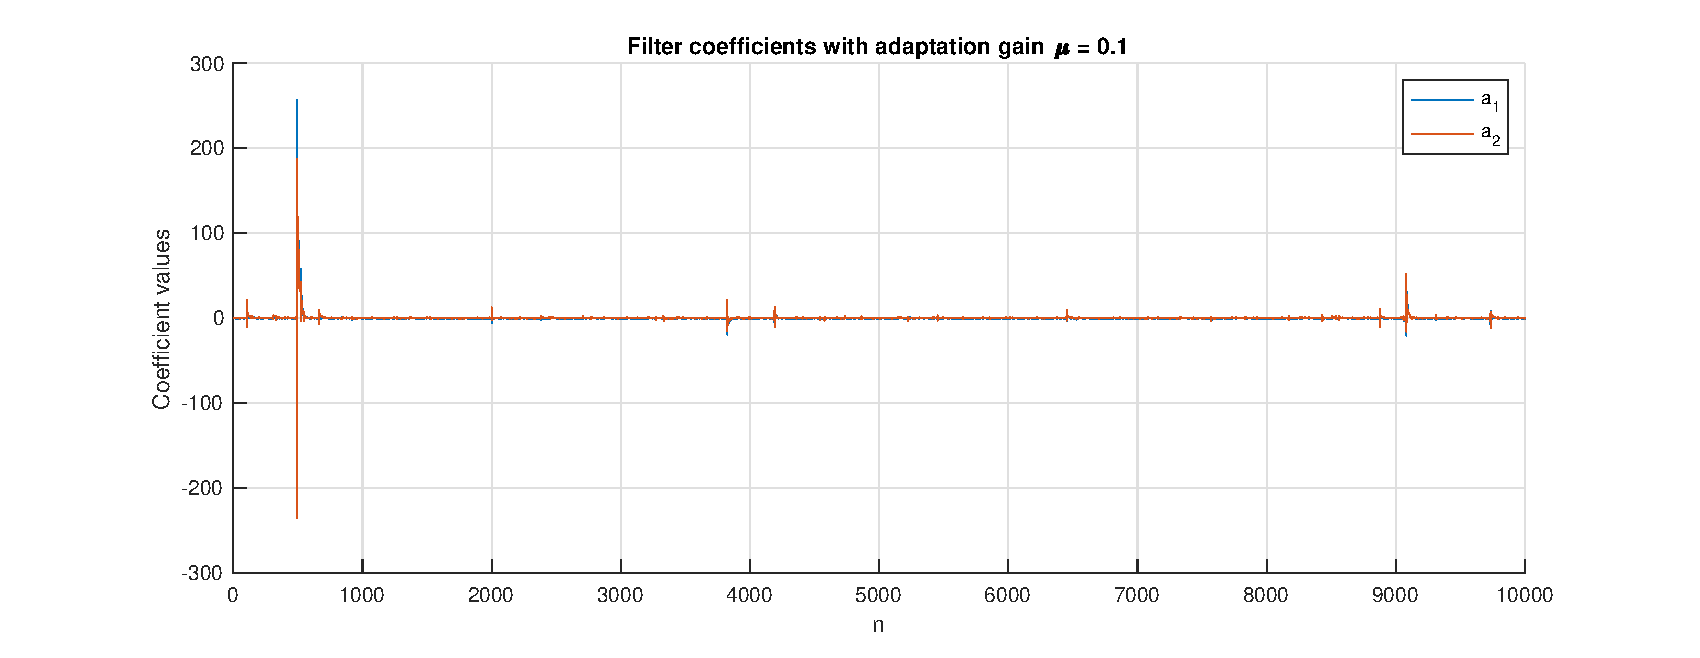
\includegraphics[width=\linewidth]{assignment4figs/armu01.eps}  
  \caption{Adaptation gain $\mu = 0.1$.}
\end{subfigure}
\caption{Coefficient evolution for given system using \code{lms()} and variable adaptation gain $\mu$.}
\label{fig:mu2}
\end{figure}

\noindent
An adaptation gain of $0.001 \leq \mu \leq 0.01$ appears to strike a balance between fast convergence but minimal distortion and therefore more stability.

% 4.5  Speech recognition
\subsection{Speech recognition}

The AR system given can be used to estimate the model order for best prediction performance for 5 audio snippets. These snippets contain my voice saying the letters 'E', 'A', 'S', 'T' and 'X'. Figure \ref{fig:letter_e} shows the original signal for the letter 'E'.

\begin{figure}[H]
    \centering
    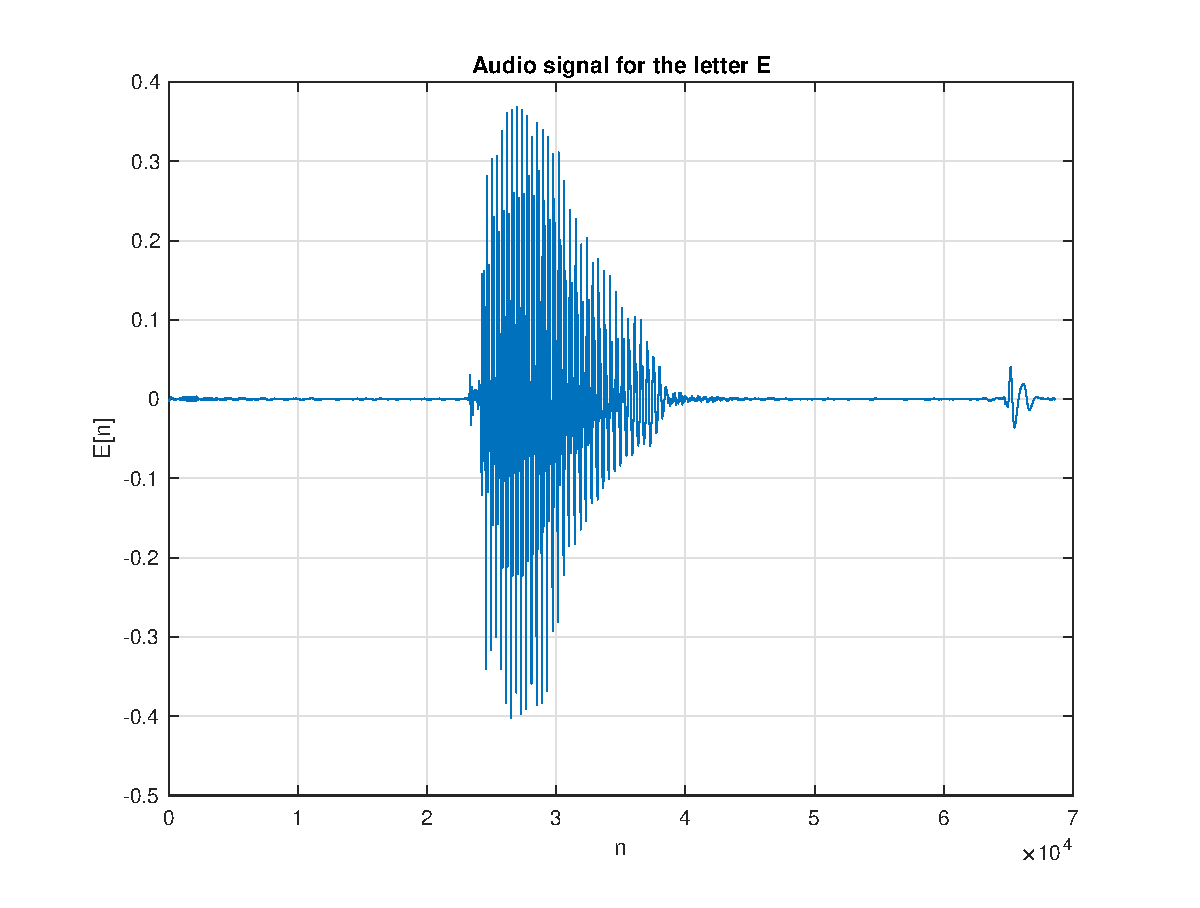
\includegraphics[width=8cm]{assignment4figs/e.eps}
    \caption{Audio signal of my voice saying 'E'.}
    \label{fig:letter_e}
\end{figure}

\noindent
In order to determine the model order of each signal, the $AIC$ and $MDL$ were calculated for each and their global minima were found. The results are displayed in Table \ref{Tab:aestx}.

\begin{table}[H]
\centering
\begin{tabular}{C{4cm} C{1cm} C{1cm} C{1cm} C{1cm} C{1cm} }
\Xhline{2\arrayrulewidth}
\textbf{Measure} & \multicolumn{5}{c}{\textbf{Letter}}\\
\textcolor{white}{.}  & E & A & S & T & X          \\\Xhline{2\arrayrulewidth}
\textbf{AIC} & 3 & 2 & 11 & 6 & 12 \\\Xhline{2\arrayrulewidth}
\textbf{MDL} & 2 & 2 & 7 & 5 & 10\\\Xhline{2\arrayrulewidth}
\end{tabular}
\caption{Statistics for different audio signals.}
\label{Tab:aestx}
\end{table}

\noindent
The Wiener coefficients were calculated using the same method before, and their evolution is shown in Figure \ref{fig:evolution}. Gear shifting was not used because the signals are non-stationary.



\begin{figure}[H]
\begin{subfigure}{.32\textwidth}
  \centering
  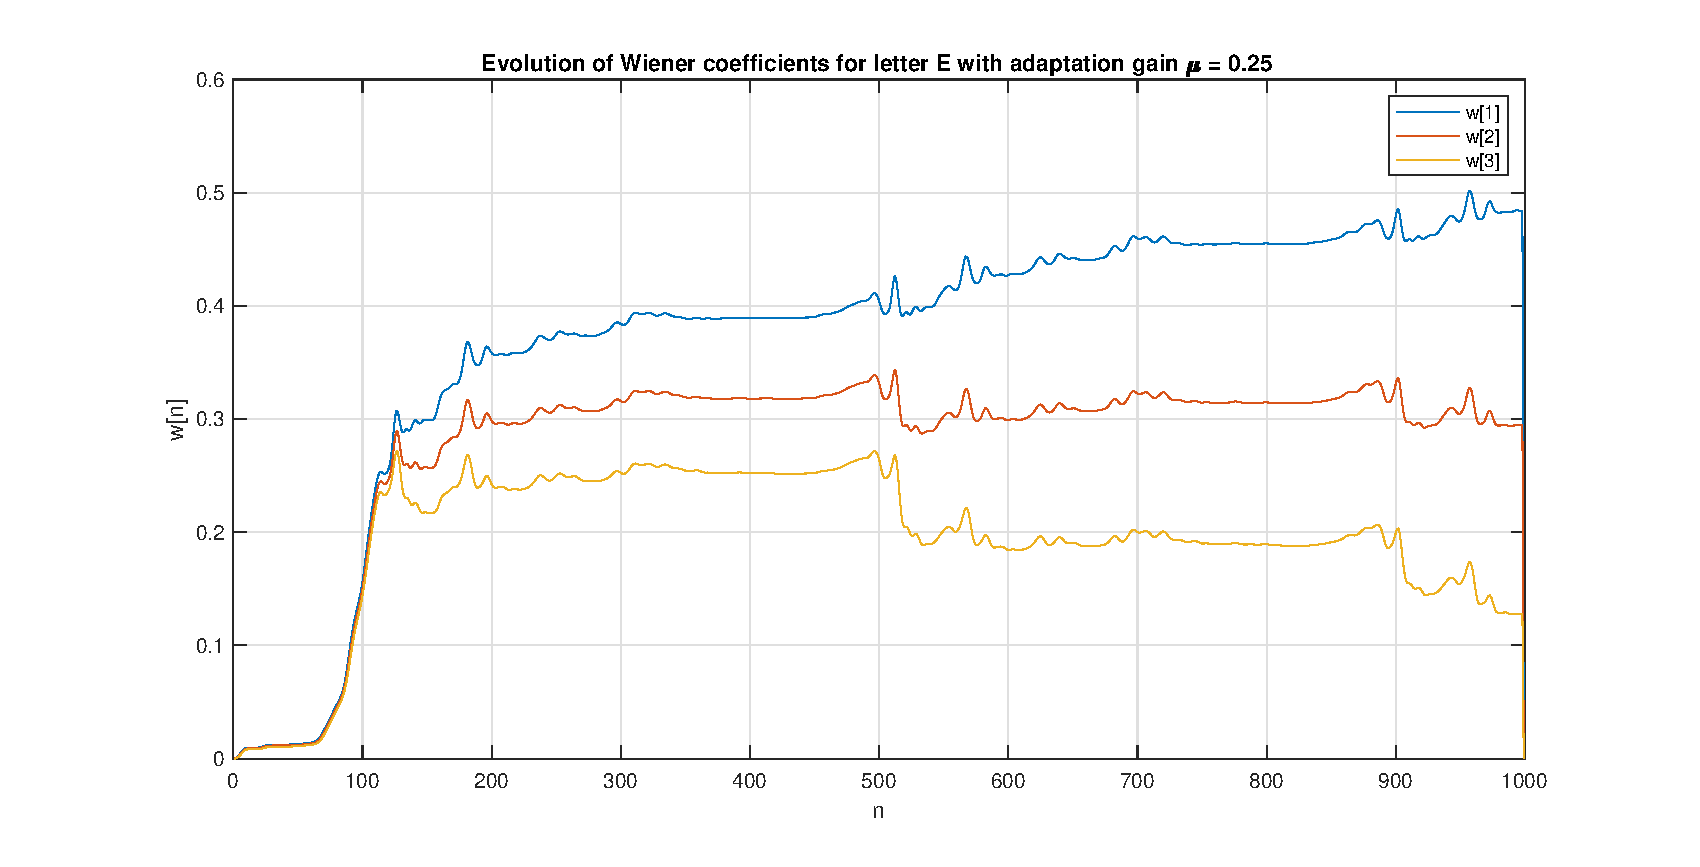
\includegraphics[width=\linewidth]{assignment4figs/wienerE.eps}  
  \caption{Letter E.}
\end{subfigure}
\begin{subfigure}{.32\textwidth}
  \centering
  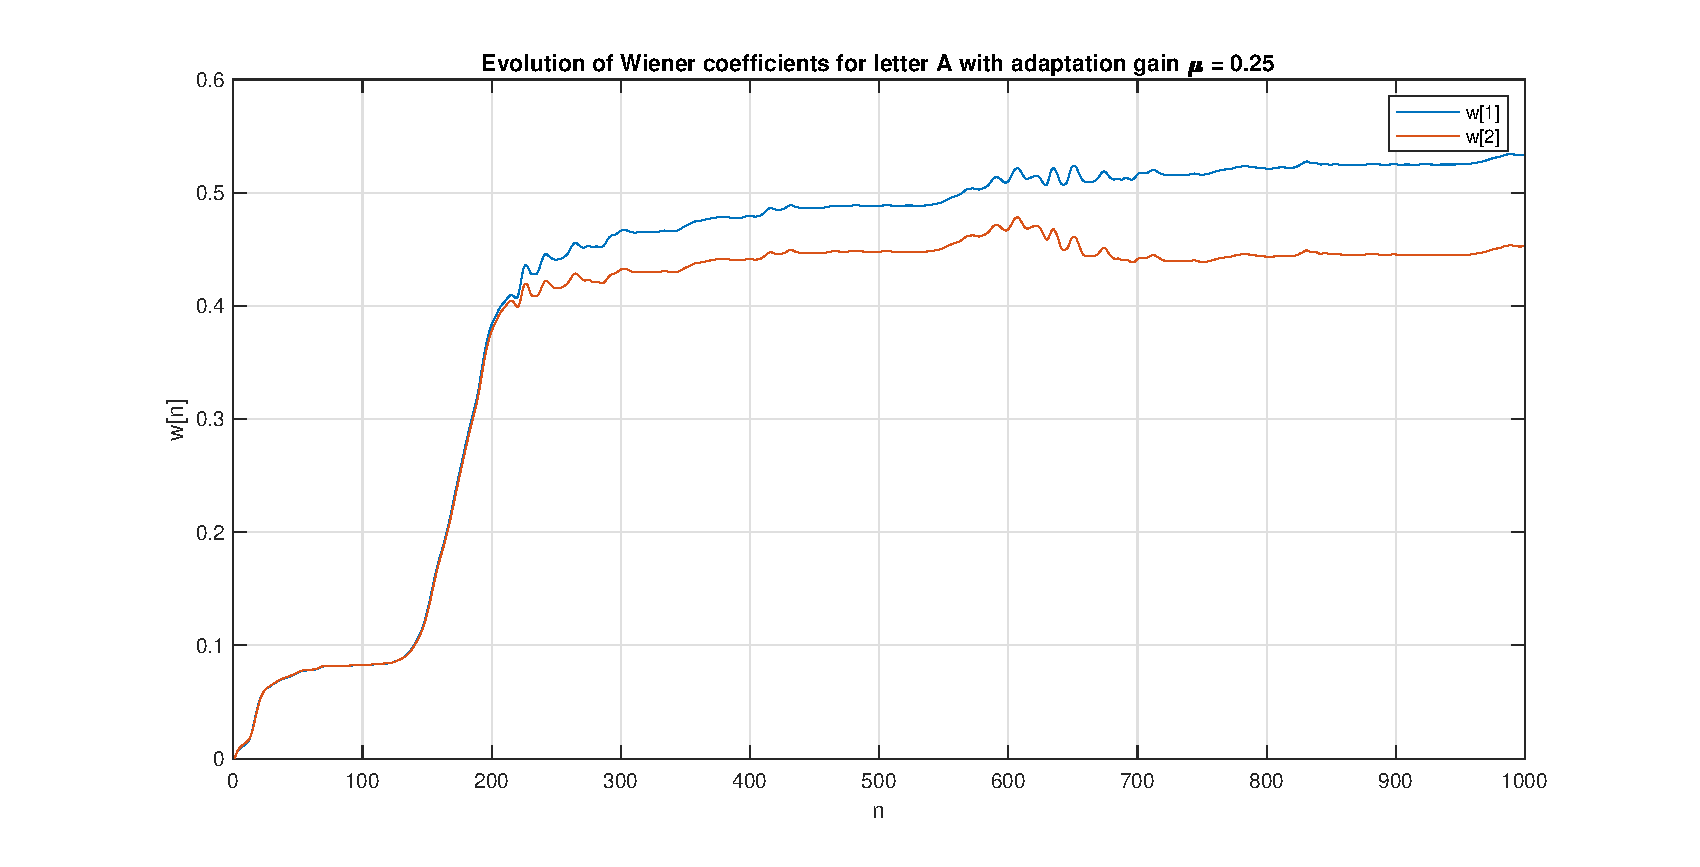
\includegraphics[width=\linewidth]{assignment4figs/wienerA.eps}  
  \caption{Letter A.}
\end{subfigure}
\begin{subfigure}{.32\textwidth}
  \centering
  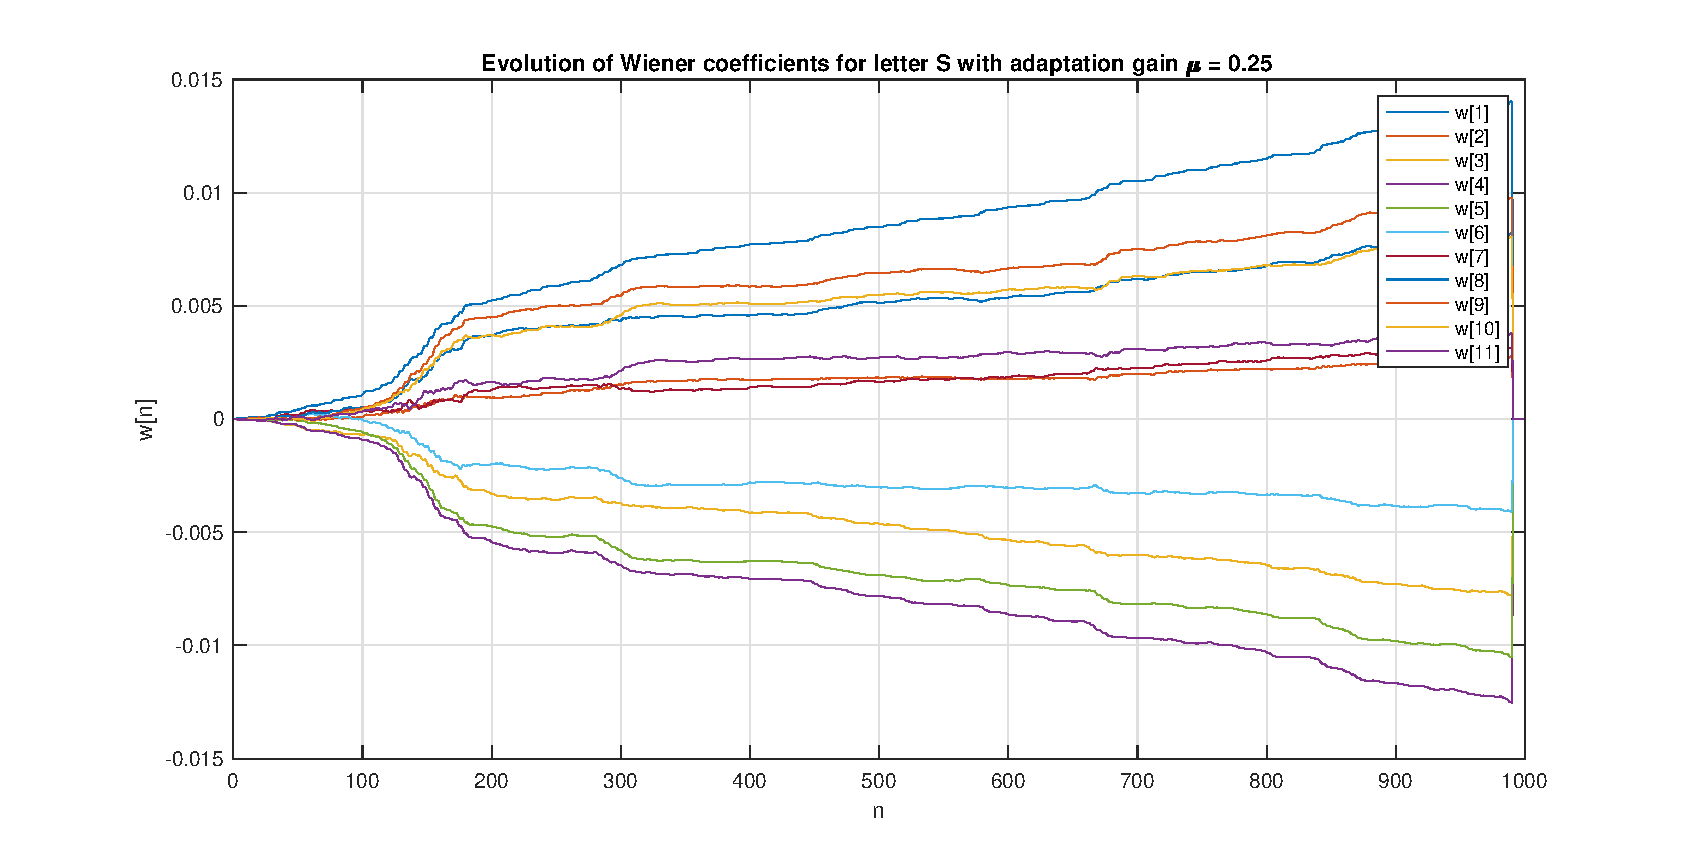
\includegraphics[width=\linewidth]{assignment4figs/wienerS.eps}  
  \caption{Letter S.}
\end{subfigure}\\
\begin{center}
\begin{subfigure}{.32\textwidth}
  \centering
  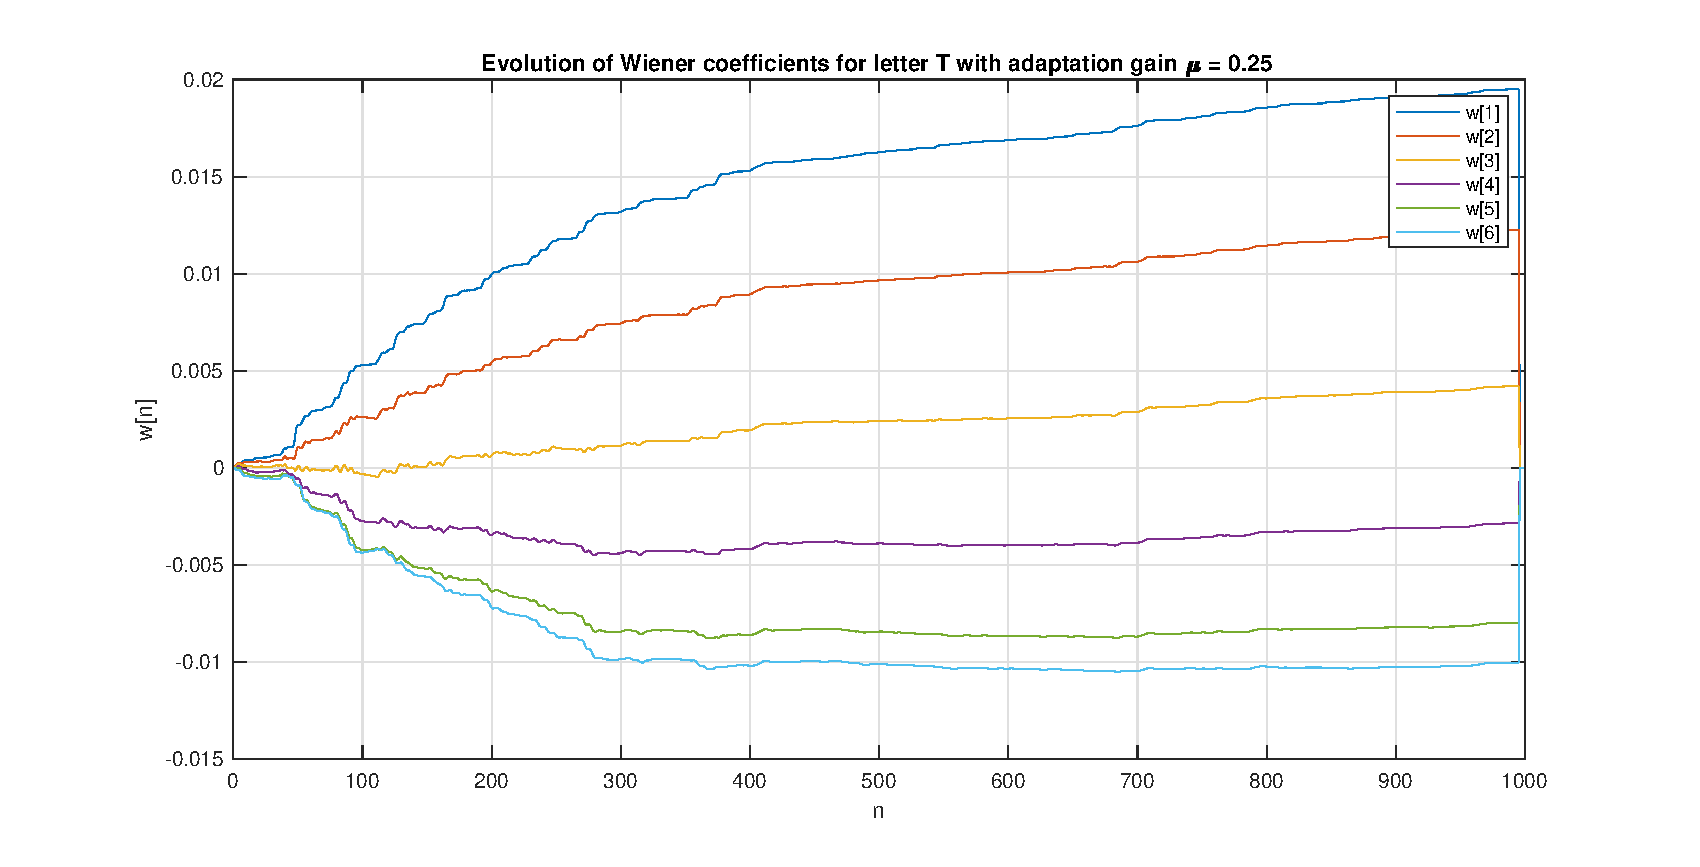
\includegraphics[width=\linewidth]{assignment4figs/wienerT.eps}
  \caption{Letter T.}
\end{subfigure}
\begin{subfigure}{.32\textwidth}
  \centering
  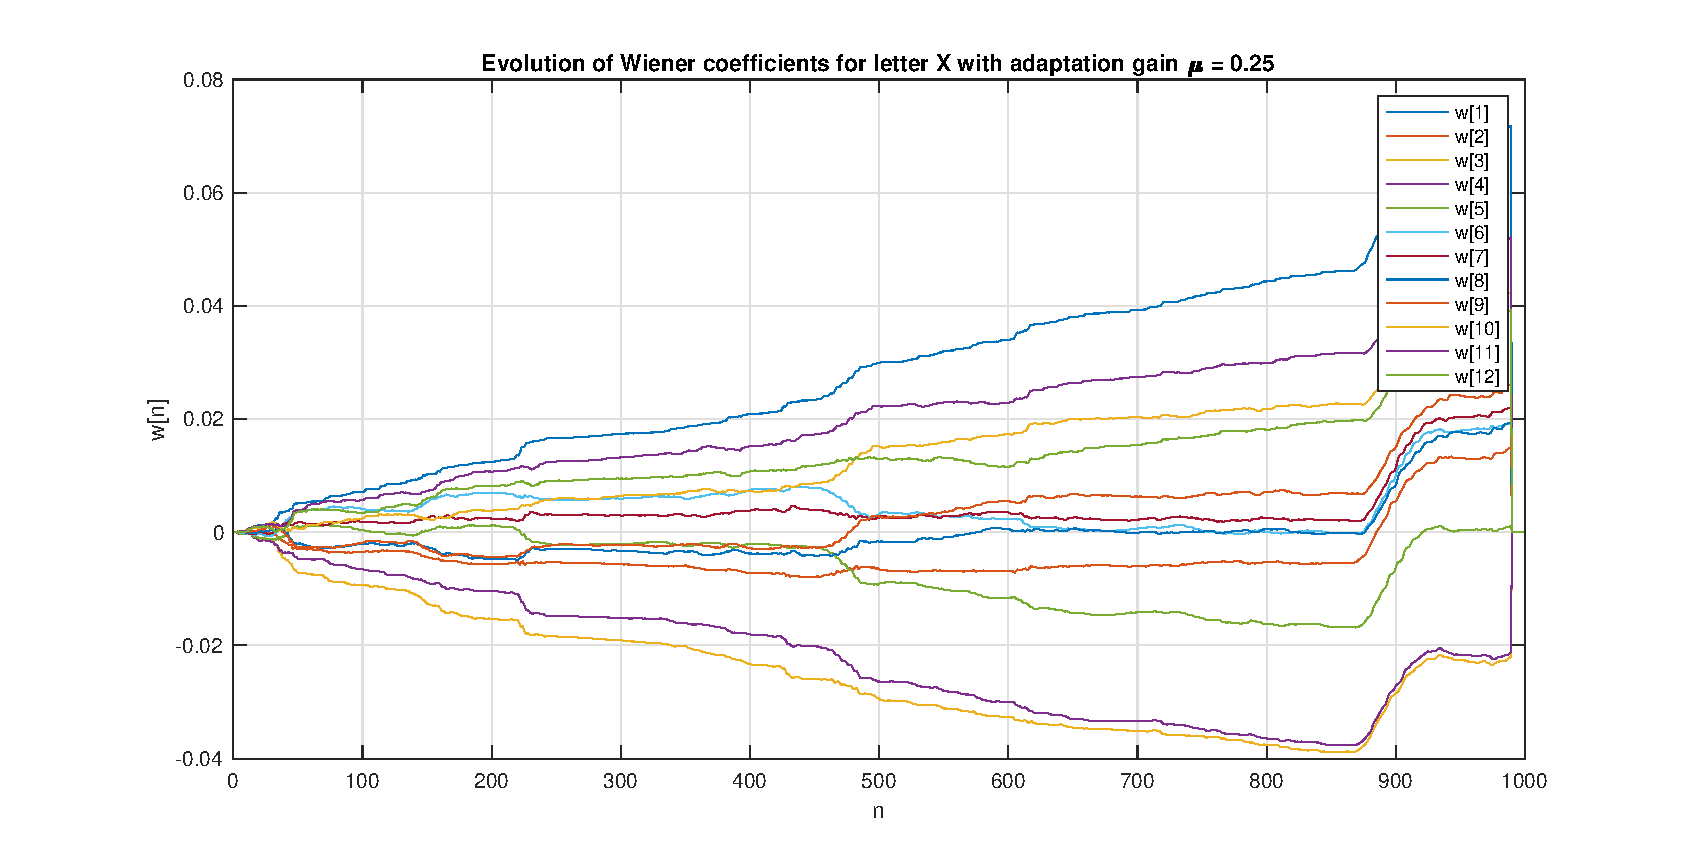
\includegraphics[width=\linewidth]{assignment4figs/wienerX.eps}  
  \caption{Letter X.}
\end{subfigure}
\end{center}\\
\caption{Evolution of coefficients for different audio signals.}
\label{fig:evolution}
\end{figure}


% 4.6  Dealing with computational complexity: sign algorithms
% \subsection{Dealing with computational complexity: sign algorithms}

% Due to the computational complexity of the LMS algorithm, it is often implemented using less complex sign algorithms, as described by Equations \ref{eqn:sign1}-\ref{eqn:sign3}.

% \begin{equation}
% \text {signed-error: } & \mathbf{w}(n+1)=\mathbf{w}(n)+\mu \operatorname{sign}(e[n]) \mathbf{x}(n)
% \label{eqn:sign1}
% \end{equation}
% \begin{equation}
% \text {signed-regressor: } & \mathbf{w}(n+1)=\mathbf{w}(n)+\mu e[n] \operatorname{sign}(\mathbf{x}(n))
% \label{eqn:sign2}
% \end{equation}
% \begin{equation}
% \text {sign-sign: } & \mathbf{w}(n+1)=\mathbf{w}(n)+\mu \operatorname{sign}(e[n]) \operatorname{sign}(\mathbf{x}(n))
% \label{eqn:sign3}
% \end{equation}

% \noindent
% I wrote a MATLAB script to implement these algorithms and compared the convergence of coefficients with the standard LMS algorithm. The results are shown in Figure \ref{fig:coeffs2}.

% \begin{figure}[H]
% \centering
% \begin{subfigure}{.45\textwidth}
%   \centering
%   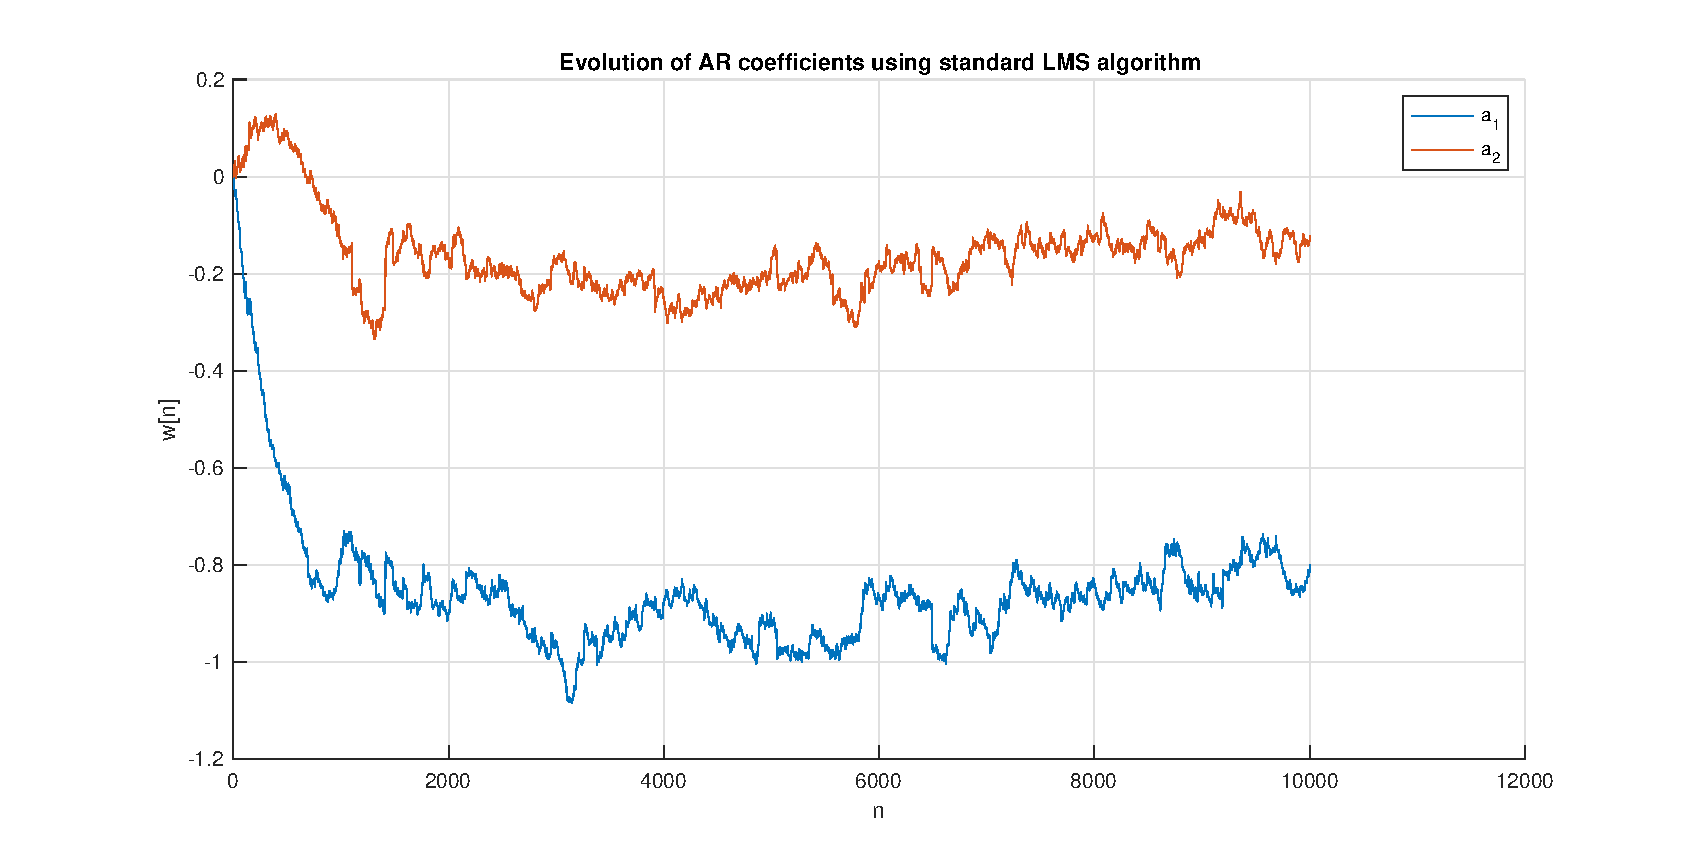
\includegraphics[width=\linewidth]{assignment4figs/standard.eps}
%   \caption{Standard LMS.}
% \end{subfigure}
% \begin{subfigure}{.45\textwidth}
%   \centering
%   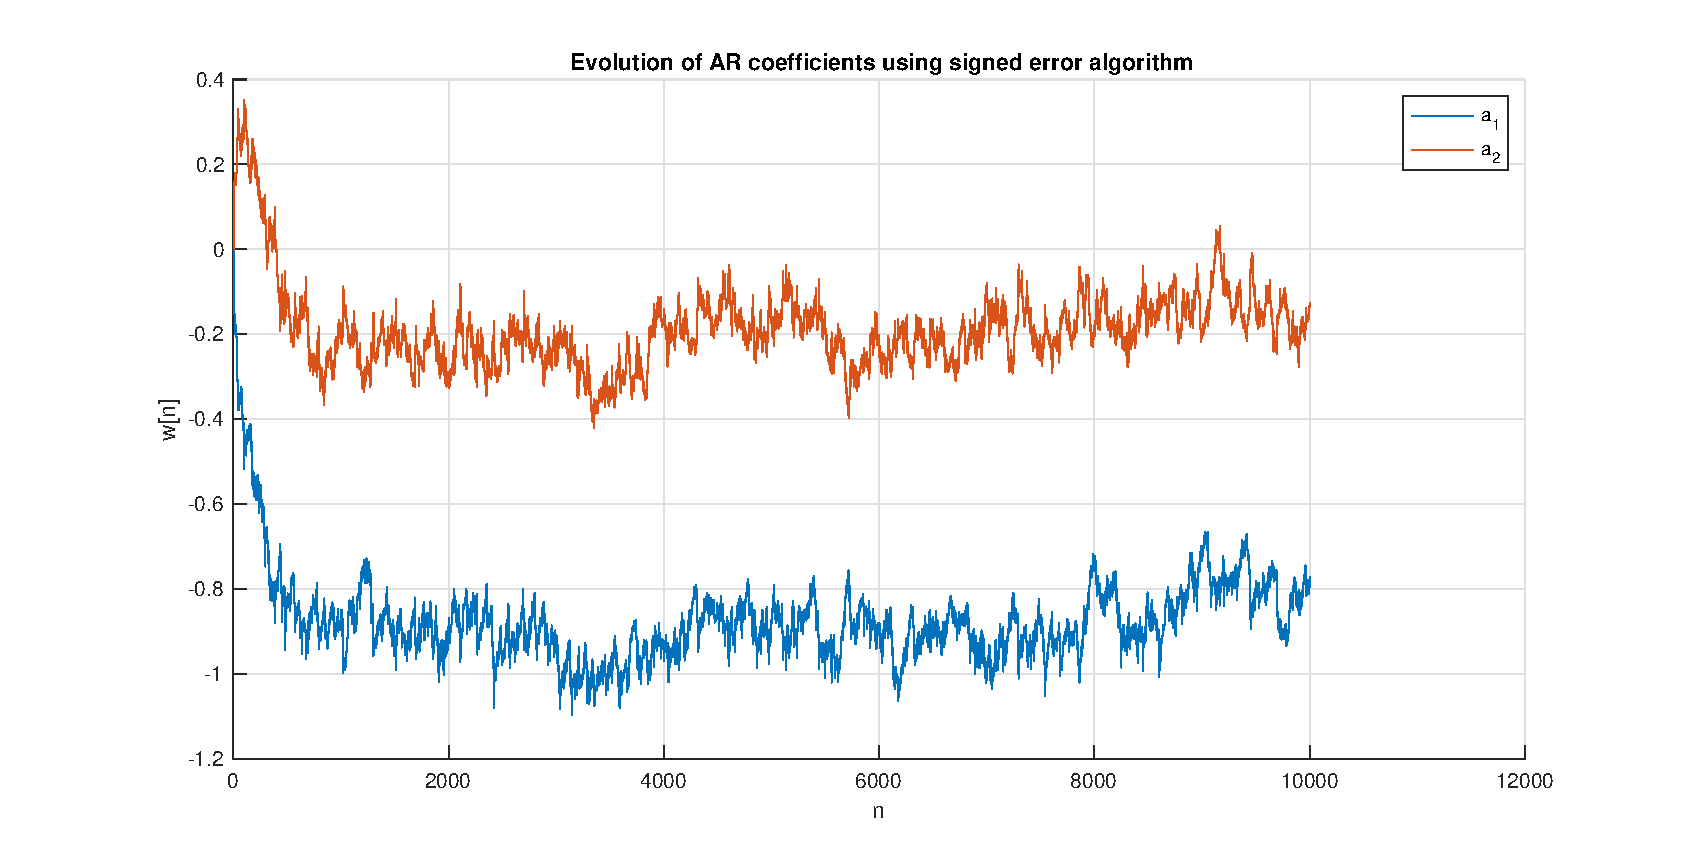
\includegraphics[width=\linewidth]{assignment4figs/signerr.eps} 
%   \caption{Signed-error.}
% \end{subfigure}\\
% \begin{subfigure}{.45\textwidth}
%   \centering
%   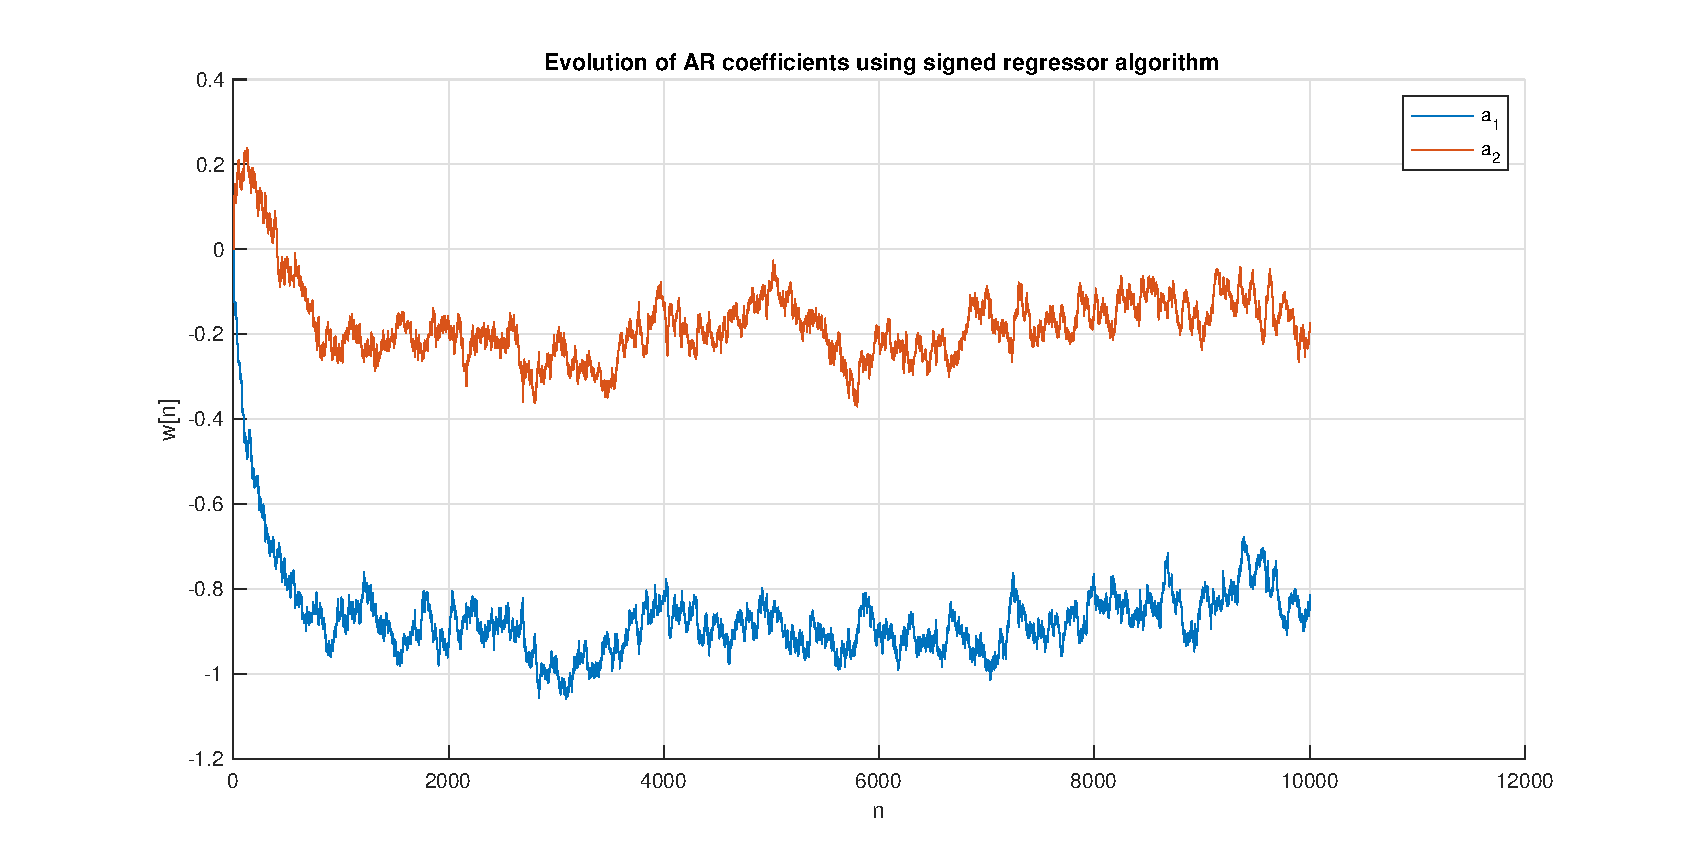
\includegraphics[width=\linewidth]{assignment4figs/signreg.eps} 
%   \caption{Signed-regressor.}
% \end{subfigure}
% \begin{subfigure}{.45\textwidth}
%   \centering
%   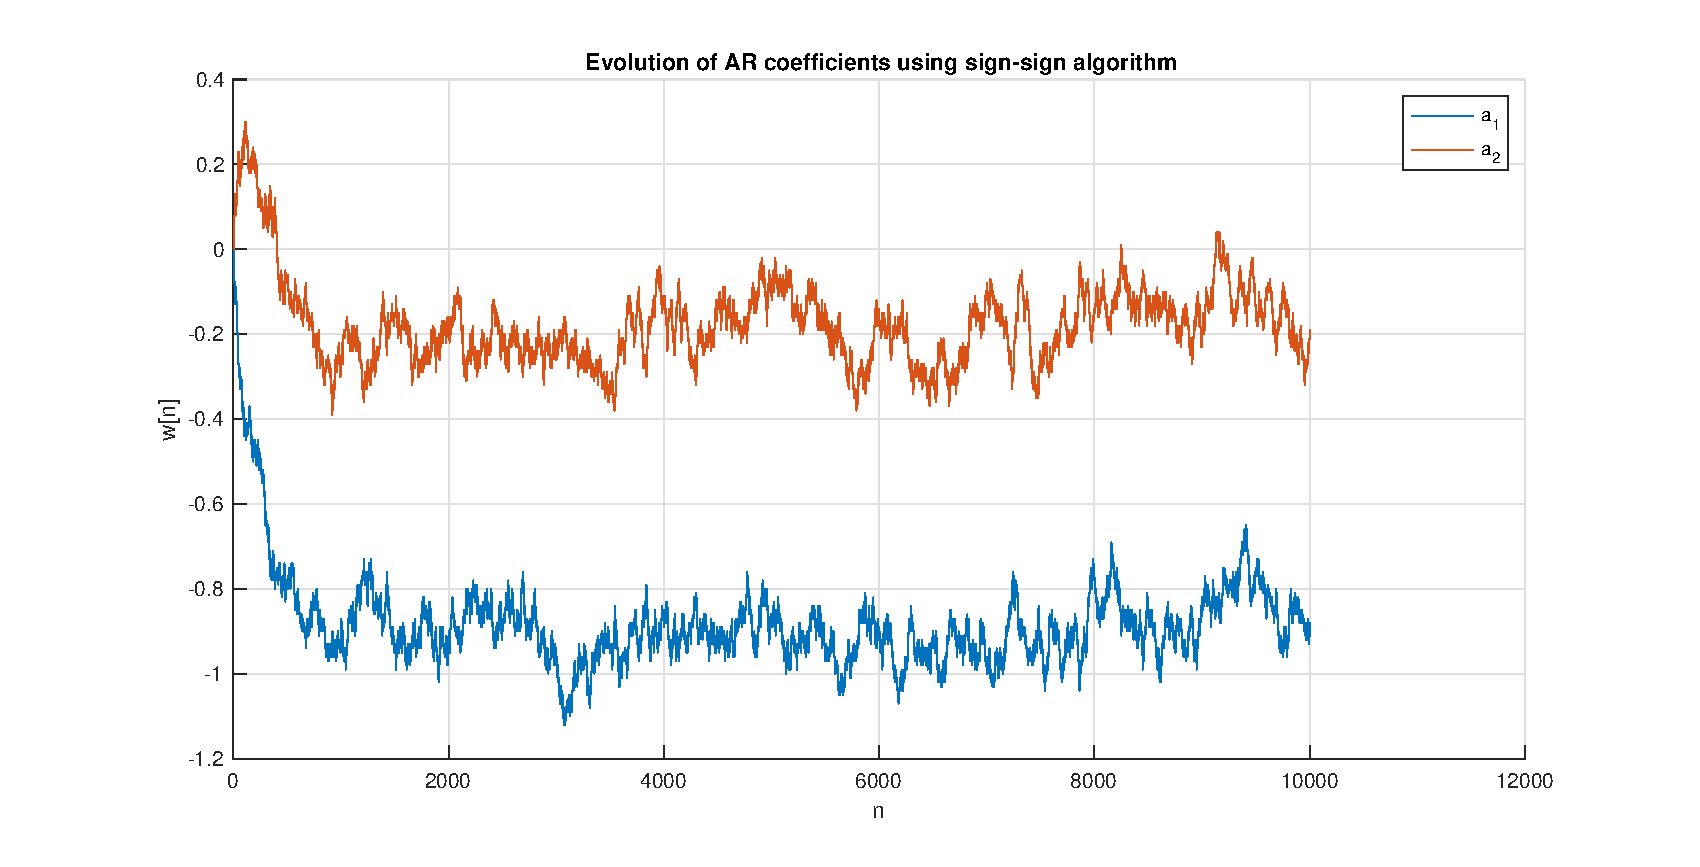
\includegraphics[width=\linewidth]{assignment4figs/signsign.eps}  
%   \caption{Sign-sign.}
% \end{subfigure}
% \caption{Coefficient evolution for standard and signed LMS algorithms.}
% \label{fig:coeffs2}
% \end{figure}

% \noindent
% The sign algorithms have the effect of increasing the variance of the coefficient evolution, but in some cases improve the convergence time. For example, the signed-error algorithm clearly leads to faster convergence than the standard LMS algorithm.